This section is focused on the audio properties of the PD patch and the control structures which operate them specifically. In addition to this, many different general-purpose control objects were created to streamline development. A full glossary is available in appendix \ref{x:glossary}, page \pageref{x:glossary}.

The synthesiser is configured as a parallel formant synthesiser with an adjustable LF-model of the glottal flow derivative as the sound source. Aspiration and frication noise are provided by two additional noise generators in the voice source. Pseudo-random flutter is implemented using Klatt's algorithm detailed in the previous section. The formants are modelled as band-pass filters with adjustable gain, centre frequency and bandwidth. The signal path is for this system is outlined in the signal flow diagram in Figure \ref{fig:signal_path} below.
%
\begin{figure}[H]
	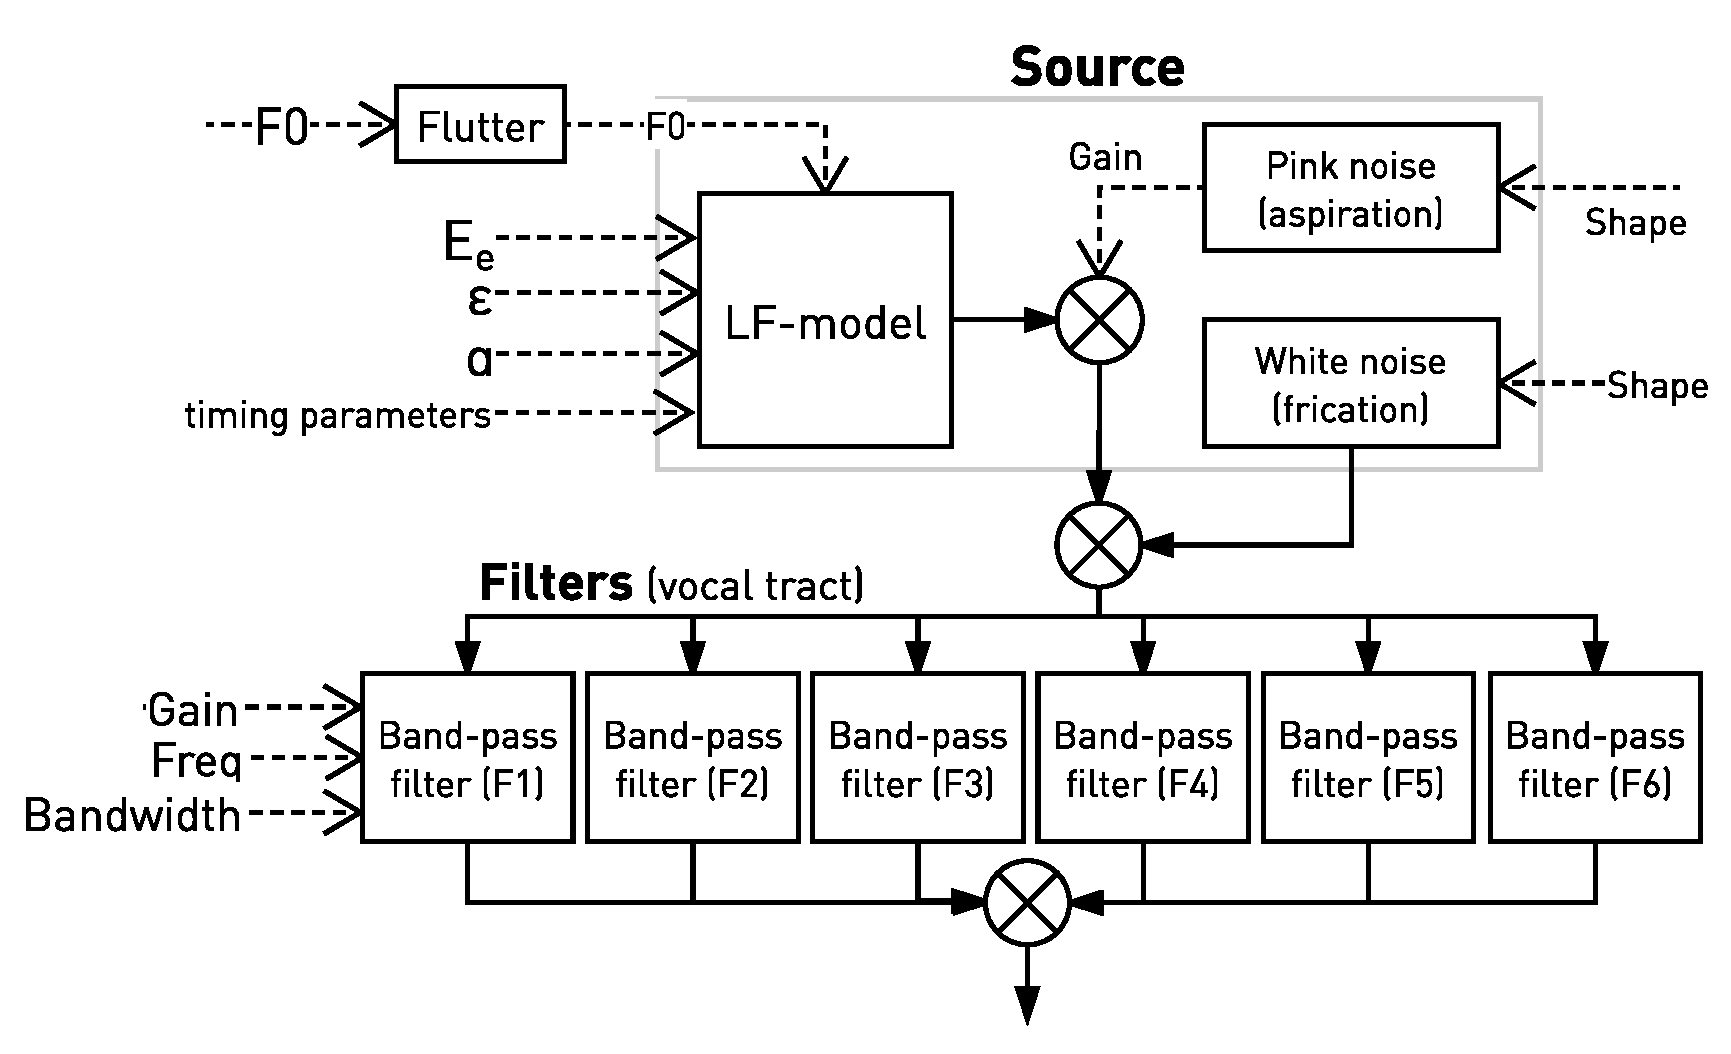
\includegraphics[width=0.5\textwidth]{signal_flow.pdf}
	\caption{Signal path diagram for the system. Audio signals are represented with black arrows, control signals are represented with dotted arrows.}
	\label{fig:signal_path}
\end{figure}
%
In the top-level patch the connecting edges of the objects are reserved only for audio signals to make the data flow clear (see Figure \ref{fig:top_level} below). Control signals are routed using message receivers.

I initially used a large number of formants (10). This did create added realism but put a lot of burden when trying to make adjustments. Fant \cite{Fant1995} cites a formula
%
\begin{equation}
	m = F_s(l_e / c)
\end{equation}
%
which defines the minimum number of VTTF poles required to maintain correct spectral distribution for cascade formant synthesis. Assuming an average male vocal tract length of $l_e=17.65\si{5cm}$ and a sampling rate of $F_s = \si{44100Hz}$ this indicates a need for 22 formants. This seems well beyond what is likely to be practical to implement in PD, although the figure is for cascade rather than parallel formant synthesis so further reading is needed. I reduced my system to four formants and added a fifth to model an additional prominent formant movement in the diphthong of my chosen word.
%
\begin{figure}[H]
	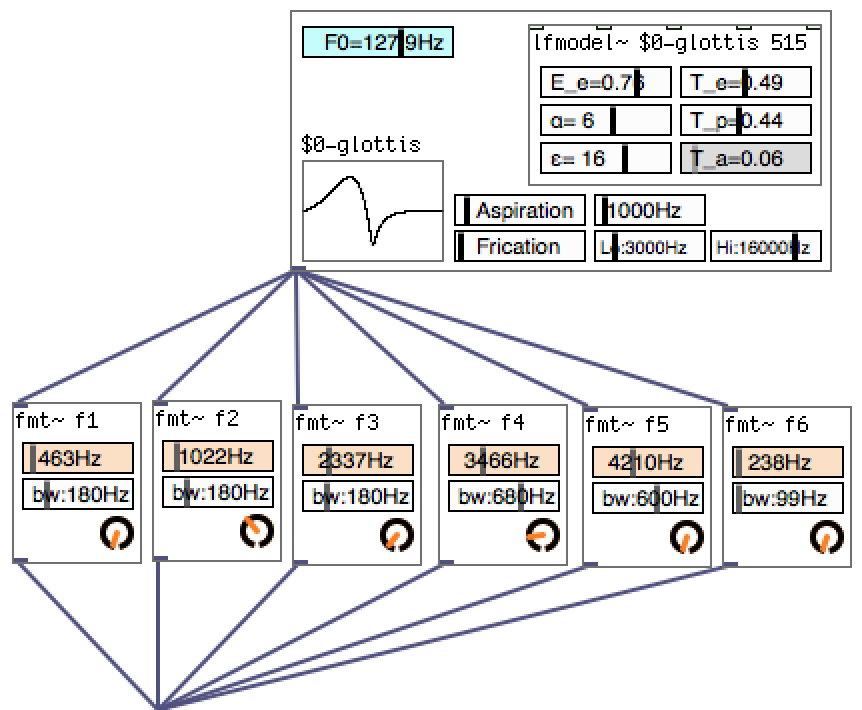
\includegraphics[width=0.5\textwidth]{top_level.png}
	\caption{Signal flow in the PD patch: from sound source through the vocal tract}
	\label{fig:top_level}
\end{figure}
%
In order to recreate the spectrum more precisely I had to use more configurable filters than the standard array of \obj{bp\~}, \obj{lop\~} and \obj{hip\~}. I found for the high and low-pass filters especially that the rolloff was too gradual to be of much use. Instead I used the built-in \obj{biquad\~} filter using \obj{bandpass} to calculate the coefficients for the formants. This object specifies the bandwidth in octaves so I created some logic to convert to a bandwidth in Hertz to make adjustments quicker. However it does not map the centre frequency precisely because \obj{bandpass} sets the bandwidth logarithmically rather than linearly. 

A controller patch (\filename{controller.pd}, Figure \ref{fig:controller} below) has any array of buttons for different phonemes and words, and when they are pressed sends control messages to the vocal tract and voice source patches to configure them.
%
\begin{figure}[H] 
	\centering
	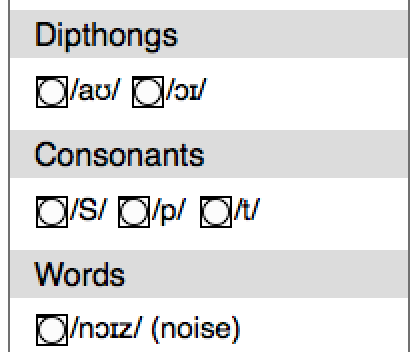
\includegraphics[height=3cm]{controller.png}
	\caption{A small section of the \obj{controller} patch showing how presets can be selected.}
	\label{fig:controller}
\end{figure}
%
For a list of the control messages see appendix \ref{x:messages} on page \pageref{x:messages}. Most control messages are terminated with an interpolation time in milliseconds; the receiver will linearly ramp to the new value in the given time. Sequencing chains of these events is handled either in \obj{qlist} objects or using a programmable message delay pipe: any global message prefixed with \msg{wait t} where $t$ is a number of milliseconds will be delayed by that time by that amount of milliseconds. For example the message \msg{wait 15 f0 100 50} would wait 15 ms before sending the message \msg{100 50} to the receiver \texttt{f0}. This behaviour is defined in \filename{msgpipe.pd} (see appendix \ref{x:glossary} for more details).

The intention to this design was to create a very flexible synthesis system that could be configured rapidly but without a lot of repetition of details. In the pursuit of naturalness it is equally important to enable a rapid turnaround of analysis of synthesis attempts, as without more sophisticated analysis techniques there is a large element of trial and error.

To that end I also created an object to allow recording directly from the synthesiser as easily as possible (see Figure \ref{fig:desk} below). Once a location has been selected with the `eject' button, pressing record will record to that file until stop is pressed.
%
\begin{figure}[H]
	\centering
	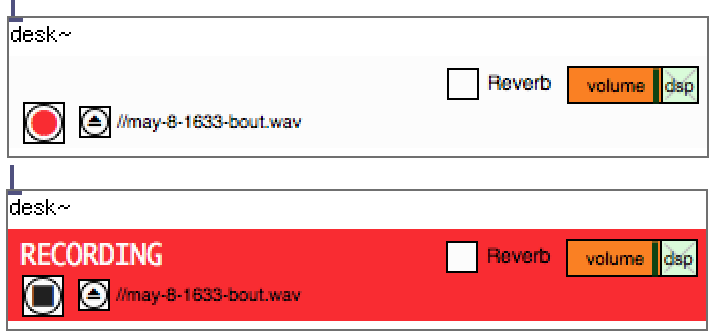
\includegraphics[width=0.45\textwidth]{desk.png}
	\caption{\obj{desk\~} object for rapidly saving samples for analysis when stopped (above) and recording (below)}
	\label{fig:desk}
\end{figure}
%

Note that analyser subpatch adapted from forum thread about log-scale graphs.